% --------------------------------------------------------------
% This is all preamble stuff that you don't have to worry about.
% Head down to where it says "Start here"
% --------------------------------------------------------------
 
\documentclass[12pt]{article}
 
\usepackage[margin=1in]{geometry} 
\usepackage{amsmath,amsthm,amssymb}
\usepackage{cite}
\usepackage{url}


%for code listings%
\usepackage{listings}
\usepackage{color}
\usepackage{graphicx}

\definecolor{dkgreen}{rgb}{0,0.6,0}
\definecolor{gray}{rgb}{0.5,0.5,0.5}
\definecolor{mauve}{rgb}{0.58,0,0.82}

\setlength{\parskip}{\baselineskip}%
\setlength{\parindent}{0pt}%

\lstset{frame=tb,
	language=C++,
	aboveskip=3mm,
	belowskip=3mm,
	showstringspaces=false,
	columns=flexible,
	basicstyle={\small\ttfamily},
	numbers=none,
	keywordstyle=\color{blue},
	identifierstyle = \color{dkgreen},
	commentstyle=\color{gray},
	stringstyle=\color{mauve},
	breaklines=true,
	breakatwhitespace=true,
	tabsize=5
}

 
\newcommand{\N}{\mathbb{N}}
\newcommand{\Z}{\mathbb{Z}}
 
\newenvironment{theorem}[2][Theorem]{\begin{trivlist}
\item[\hskip \labelsep {\bfseries #1}\hskip \labelsep {\bfseries #2.}]}{\end{trivlist}}
\newenvironment{lemma}[2][Lemma]{\begin{trivlist}
\item[\hskip \labelsep {\bfseries #1}\hskip \labelsep {\bfseries #2.}]}{\end{trivlist}}
\newenvironment{exercise}[2][Exercise]{\begin{trivlist}
\item[\hskip \labelsep {\bfseries #1}\hskip \labelsep {\bfseries #2.}]}{\end{trivlist}}
\newenvironment{reflection}[2][Reflection]{\begin{trivlist}
\item[\hskip \labelsep {\bfseries #1}\hskip \labelsep {\bfseries #2.}]}{\end{trivlist}}
\newenvironment{proposition}[2][Proposition]{\begin{trivlist}
\item[\hskip \labelsep {\bfseries #1}\hskip \labelsep {\bfseries #2.}]}{\end{trivlist}}
\newenvironment{corollary}[2][Corollary]{\begin{trivlist}
\item[\hskip \labelsep {\bfseries #1}\hskip \labelsep {\bfseries #2.}]}{\end{trivlist}}
 
\begin{document}
 
% --------------------------------------------------------------
%                         Start here
% --------------------------------------------------------------
 
%\renewcommand{\qedsymbol}{\filledbox}
 
\title{Advanced Multiprocessor programming \\ Group Project}%replace X with the appropriate number
\author{Nick Mayerhofer (0726179), Konrad Pozniak (0925996)\\ %replace with your name
} %if necessary, replace with your course title
 
\maketitle

% --------------------------------------------------------------
%                  Start our Content here
% --------------------------------------------------------------

%zu finden mit einem Klick auf "PROJECT" links oben...
\section{Project Description}

In this project we are going to implement four different list-based sets and try to find out which one has the best performance properties, in a highly parallel program. This includes testing the implementations for correctness and creating our own meaningful benchmarks. 

We assume the reader is familiar with the lecture \cite{traeffSlides}.

\subsection{Programming language and environment}
For this project, we use C++ 11 and its native thread implementation.
Our benchmark tests are run on two shared memory multicore machines of Vienna university of technologies parallel computing research group:

\begin{itemize}
  \item Mars\\
  8 Intel Xeon E7-8850 CPUs with 10 Cores @ 2Ghz\\
  160 Threads\\
  1 TiB RAM\\
  Debian GNU/Linux 3.14-1-amd64
  \item Ceres\\
  4 SPARC T5 CPUs with 16 Cores @ 3.6Ghz\\
  512 Threads\\
  1 TiB RAM\\
  Oracle Solaris 11
\end{itemize}
All test and benchmark programms are compiled with the GNU C++ compiler \texttt{g++} (version 4.9.2 on Mars and 4.8.2 on Ceres) and full optimization (\texttt{-O3}) for 64 bit (\texttt{-m64}) with C++11 standard (\texttt{-std=c++11}).

\section{The Set data type} 
A set is a data type that can contain certain values, without any particular order, and no repeated values. It is a computer implementation of the mathematical concept of a finite set. Unlike most other collection types, rather than retrieving a specific element from a set, one typically tests a value for membership in a set. \cite{journals/ipl/Hehner81}\\
In this project we will take a look at the three most important operations of a set:

\begin{itemize}
  \item \texttt{bool add(long item)}\\
  	Adds an item to the set.\\
	Returns true if successfull, false if the item already was in the set.
  \item \texttt{bool remove(long item)}\\
  	Removes an item from the set.\\
	Returns true if successfull, false if the item was not in the set.
  \item \texttt{bool contains(long item)}\\
  	Checks if an item is contained in a set.\\
	Returns true if the item is contained, false if not.
\end{itemize}

\subsection{Reference Set}
As reference implementation we used \texttt{std::set} from the C++ standard library and synchronized each call to the object with a global \texttt{std::mutex} lock, since it is not thread safe.

This construction is deadlock free, since there is only one global lock. \texttt{std::mutex} has no guarantees to be starvation free or fair, so this set also has no guarantees. The linearization point is trivially where the lock is acquired.

The c++11 implementation of \texttt{std::set} is based on a binary search tree, while our implementations will be based on simple linked lists. Thus it is interesting to see how much of a difference this makes. If the set is filled with many elements, the time needed to search for an element will certainly be noticeable. We also expect that this reference set will be much faster on a single thread than our implementations, but the global lock will probably slow it down very much in parallel mode.

Following are explanations of the four different implementations, introduced in the lecture \cite{traeffSlides}. After that we are going to explain how we are going to penetrate the implementation, in order to test them.
\subsection{Fine-Grained Locking}
Instead of a global lock this implementation has a lock for each individual node, s.t. multiple threads can operate at the same time on different locations of the list.

The set with fine grained locking is deadlock free, since locks are always acquired in the same order. But it has no progress guarantees. The linearization point with an item is in the set, is when the corresponding node is locked. Otherwise when the next higher node is locked.

Implementing this set was pretty straightforward, except we found a little mistake in the lecture slides, see \ref{mistakes}.

\subsection{Optimistic Synchronization}
Optimistic synchronization does not lock any nodes when searching for an element. It locks just if element has been found, the searched element itself and its predecessor. This requires validation that the nodes are still linked into the list after they got locked. If not, the process has to be restarted - this might be a performance problem.

As with the fine grained locking set, this set has no progress guarantees. The operation linearize when the node or the next higher node is successfully validated.

\subsection{Lazy Synchronization}
Lazy synchronization does not acquire locks for a \texttt{contains} call, in contrast to optimistic synchronization. To counteract the possibility that \texttt{contains} returns a element that has been unlinked from the list, each node can be marked as removed with a flag. It is then logically removed from the set, while it may be still linked into the list. This leads to the problem, that nodes cannot be deleted safely, even after they have been unlinked - other threads might still be accessing them. See \ref{memoryleak} for possible solutions to this.

We expect this implementation to have better performance than the previous ones, because \texttt{contains} does not need any locks and is wait free, and \texttt{validate} does not need to iterate through the whole list again.

\subsection{Lock Free}
The lock free implementation does not use any locks, but atomic operations with hardware support to update the pointers in the list. The marked flag and the pointer need to be treated as one atomic unit, though.

Pointer on AMD64 have 48 bit, but are aligned to 64 bit in memory \cite[p. 120]{amd64ArchManual}. The same is true for the SPARC T5 architecture. It is possible to use one of the surplus bits as marked flag, so the flag and the pointer can be moved together in a single compare-and-swap operation. 

This was quite tricky to implement, since dereferencing a pointer when the flag is set leds to an memory access violation. So before every pointer dereferentiation the flag has to be removed, but it must not be forgotten when linking nodes in the list. 

We used the GCC builtin \texttt{bool \_\_sync\_bool\_compare\_and\_swap (type *ptr, type oldval type newval, ...)}. This builtin directly translates to a single assembler instruction and should be the fastest compare and swap available. Of course it is still is a memory fence and can be very costly.

Since the marked flag is part of the pointer to the next node, one must be very careful when unlinking nodes in \texttt{remove} or \texttt{find}: Just swapping the pointers can override the flag of the predecessor node. See \ref{mistakes} for a detailed description.

The lock free set is completely lock free, \texttt{contains} is even wait free. We expect the lock free set to perform best in our benchmarks because of this properties of lock freenes.


\section{Testing for correctness}
To test our implementations, we designed some testcases to make sure they run correct.

The first test case lets all threads \texttt{insert} the same elements multiple times, then checks that for each elements \texttt{add} returned \texttt{true} only once, and that all elements are really in the set. Then all threads \texttt{remove} the same elements again, and for each element, \texttt{remove} must only return \texttt{true} once. After the tests, the set must be empty.

The second test case mixes the three operations and aims to find any bugs caused by sideeffects between the operations.

With these testcases we were able to find mistakes in the example code from the lecture slides and correct them. See \ref{mistakes} for a detailed description.

All tests have been run correctly at least 100 times each on both testing machines, Saturn and Ceres, with all our set implementations and different number of elements and threads.
\section{Benchmark}
We tried to construct the Benchmark environment as generic as possible, to fulfill each of our following requirements:
\begin{itemize}
\item Encapsulate as much as possible in reusable code
\item Be as precise as possible (e.g. give the threads themselves the ability to execute their time measurements to keep the overhead low)
\item Benchmark each operation separately, namely: add, contains, remove
\item Output the results to files to keep the possibility for log outputs alive
\end{itemize}

To make sure we use the most efficient time measurement, we tested all available functions for their performance, see figure \ref{timer_benchmark}. We then decided to use the standard C++ high precision clock, because its short run time and high precision. Even when calling it very often with many threads, we measured an overhead less than 50ns.

There are endless possibilities for benchmarks: All combinations of the five sets, three operations and two machines with different thread counts, iterations, datatypes, on empty or prefilled sets etc.

We created four benchmarks to measure how long a certain number of operations on a set takes, one for \texttt{add}, one for \texttt{remove}, one for \texttt{contains} and one for a combination of them. Basically every thread executes the same operations in a loop and we measured the overall time it took the threads to complete the operations. 

The \texttt{add} benchmark starts with an empty set and then every set performs 1000 insert operations on the set simultaneously. The values inserted are evenly distributed over the input space to avoid that one thread inserts only big numbers and another only small ones.

The \texttt{remove} benchmark starts with an half filled set (every second number is in the set) and then every thread performs 1000 remove operations, distributed like in the \texttt{add} benchmark, so every second \texttt{remove} fails and the set is empty at the end.

The \texttt{contains} benchmark also starts with an half filled set and then every thread performs 1000 contain operations.

In the mixed benchmark, every thread calls \texttt{add}, \texttt{contains}, \texttt{remove} and \texttt{contains} again with its thread id, so the max number of elements in the set at any time is the number of threads.


We chose 1000 as the number of iterations, because then the running time was short enough to repeat the benchmarks many times, but long enough to get meaningful measurements.


With this benchmarks we want to get a good metric for the sets performance and try to prove our hypotheses from the above set descriptions.

The results for Mars are listed in figure \ref{mars_throughput} and for Ceres in \ref{ceres_throughput}. We visualized them in figures \ref{addthrough}, \ref{containsthrough}, \ref{removethrough} and \ref{mixedthrough}.


The most obvious result is, that the fine grained locking set performs very badly on the first three benchmarks. Apparently the overhead for locking each node is much higher than the performance gain in allowing multiple threads to operate on the set at the same time. We knew the fine grained locking set would have bad performance, but we were surprised how bad it really is.

The difference between the reference set's tree implementation and our list implementation becomes visible in: the benchmarks that operate on a filled list and the advantage of the reference set is huge. On the mixed benchmark, that operates on an almost empty set, our implementations are much faster on Mars, while on Ceres only the lock free set is faster.

The throughput of the lazy synchronization set is much higher than the one of the optimistic synchronization one, especially for remove. The improvement of not locking nodes in \texttt{contains} and not iterating through the whole list again in \texttt{validate} really shows.


On Mars, the lock free set performs noticeably better than the lazy synchronization set, except in the mixed test. On Ceres, the lock free set is slower in remove and add, and faster in contains and mixed. 
Probably a compare and swap operation is more expensive on a SPARC architecture than on a AMD64 one and a locking operation conversely. Note that \texttt{contains} in both sets does not use compare-and-swap or a lock.


To measure the fairness between the threads, we let each thread run for a certain amount of time and counted the number of operations performed per thread. Our findings are presented in figure \ref{marsfairness} and \ref{ceresfairness}.

Very interesting is the difference between the two machines. On Mars, the first threads are faster than the others, because the were started before them, but overall the distribution looks pretty fair for all sets. On Ceres the plots look different. Some are really unbalanced, others less. But it is safe to say that Mars is fairer than Ceres.

We think that this difference is either caused by the different architecture of the processor or the difference in thread scheduling by the operating system.

With this knowledge we think it would be very interesting to implement a lock free set over a tree data structure to beat the performance of the reference set even on big sets.

\section{The problem with the memory leak}
\label{memoryleak}
In the lazy synchronization and lock free sets, it is not possible to determine a point where unlinked nodes can be deleted savely, because it is always possible that other threads may still be accessing the node. This causes a memory leak. We have two ideas how this problem could be solved, but we had not enough times to try them:
\begin{itemize}
  \item Using C++ smart pointer, e.g. \texttt{std::shared\_ptr}. Smart pointer automatically keep track of their memory pointees and are releasing the memory with the last pointee going out of scope. They are very convenient, but - depending on the implementation - implemented with wither locks or atomic operations and we suspect they have a bad impact on performance.
  \item Having a global memory pool managing unused nodes and instead of creating new node objects every time, reusing the old ones. This does not really prevent a memory leak, but limits the memory usage to the maximum size the set ever had. It might be a problem if nodes get reused immediately.
\end{itemize}


\section{Changes to the lecture slides} \label{mistakes}

We found some implementations in the lecture slides, not working in practice:

The first one is in the find function of the fine grained locking set.
\begin{lstlisting}
Window find (T item ) {
	Node* pred = head;
	Node* curr = pred->next;
	pred->lock();
	curr->lock();
	while (curr->item < item ) {
		pred->unlock ();
		pred = curr;
		curr = curr->next;
		curr->lock ();
	}
	return Window (pred, curr);
}
\end{lstlisting}
It is possible that a thread gets a invalid window back, because the pointer to the current node is acquired before the lock of the predecessor node. We fixed it like this:

\begin{lstlisting}
Window find (T item ) {
	Node* pred = head;
	pred->lock();
	Node* curr = pred->next;
	[...]
}
\end{lstlisting}

Another problem is in the lock free set, when a node is unlinked from the list after it has been marked. If the predecessor node is also marked, its mark is overridden by the compare and swap operation because the mark is stored in the next pointer. 

We fixed this by checking for the mark and setting it on the new pointer before the compare and swap if necessary:

\begin{lstlisting}
if(isMarked(w.curr)) {
	next = mark(next);
}		
__sync_bool_compare_and_swap(&(getPointer(w.pred)->next), w.curr, next);
\end{lstlisting}
Note: the compare\_and\_swap may be replaced through the C++11 compare and swap methods atomic::compare\_exchange\_weak \cite{cppref:compare_exchange}. Further research would


Another rare bug happened, when a node was removed from the lock free set by another thread just after \texttt{find} found it unmarked, but before it returned the node. This could cause \texttt{add} to insert an node after an removed one and return true, but the node would not be in the set. We fixed this problem by adding a check to \texttt{add}:

\begin{lstlisting}
bool LockFreeSet::add(long item) {
	LfsNode *n = new LfsNode(item, nullptr);
	while (true) {
		LfsWindow w = find(item);	
		if(isMarked(w.curr)) {
			continue;
		}
    [...]
\end{lstlisting}



%\section{Ab hier kommt beispiel Foo}

%\begin{theorem}{x.yz} %You can use theorem, proposition, exercise, or reflection here.  Modify x.yz to be whatever number you are proving
%Delete this text and write theorem statement here.
%\end{theorem}

\begin{proof}
Blah, blah, blah.  Here is an example of the \texttt{align} environment:
%Note 1: The * tells LaTeX not to number the lines.  If you remove the *, be sure to remove it below, too.
%Note 2: Inside the align environment, you do not want to use $-signs.  The reason for this is that this is already a math environment. This is why we have to include \text{} around any text inside the align environment.
\begin{align*}
\sum_{i=1}^{k+1}i & = \left(\sum_{i=1}^{k}i\right) +(k+1)\\ 
& = \frac{k(k+1)}{2}+k+1 & (\text{by inductive hypothesis})\\
& = \frac{k(k+1)+2(k+1)}{2}\\
& = \frac{(k+1)(k+2)}{2}\\
& = \frac{(k+1)((k+1)+1)}{2}.
\end{align*}
\end{proof}
 
\begin{proposition}{x.yz}
Let $n\in \Z$.  
\end{proposition}
 
\begin{proof}[Disproof]%Whatever you put in the square brackets will be the label for the block of text to follow in the proof environment.
Blah, blah, blah.  I'm so smart.
\end{proof}

 
\newpage
\section{Appendix}
The source code of this project can be found at:\\ \url{https://github.com/nickma82/advanced_multiprocessor_prog}

\begin{figure}[ht]
  \centering
\begin{tabular}{ l | c c c c }
 & add & contains & remove & mixed\\
 \hline
reference & 418.53 &  231.50 &  470.04  & 272.85\\
fine grained lock. & 17155.33 & 9360.36 & 8433.88 & 32.25 \\
optimistic sync. & 2609.88  & 418.71 & 3421.86 &   38.19\\
lazy sync. & 1333.05 &  289.80 &  215.82  &  25.22\\
lock free & 1128.28  & 161.50  & 115.61   & 29.39\\
\end{tabular}
  \caption{Average time in milliseconds of 100 throughput benchmark runs on Mars, 80 threads, each thread ran the iteration 1000 times}
  \label{mars_throughput}
\end{figure}

\begin{figure}[ht]
  \centering
\begin{tabular}{ l | c c c c }
 & add & contains & remove & mixed\\
 \hline
reference & 29.75  &  25.17  &  25.77 &   27.94 \\
fine grained lock. & 5759.07 & 6059.24 & 5886.83 & 37.72 \\
optimistic sync. & 1348.86 &  634.34 & 2344.10  &  39.79 \\
lazy sync. & 635.12  & 328.49 &  307.21  &  30.92 \\
lock free & 687.51  & 320.21 &  358.25  &  16.03\\
\end{tabular}
  \caption{Average time in milliseconds of 100 throughput benchmark runs on Ceres, 64 threads, each thread ran the iteration 1000 times}
  \label{ceres_throughput}
\end{figure}

\begin{figure}[H]
  \centering 
  \includegraphics[height=0.93\textheight]{pictures/timer_benchmarks.eps}
  \caption{average execution time of 1000 calls to different time capture methods, measured with a wrapped \textit{clock\_gettime}}
  \label{timer_benchmark}
\end{figure}

\begin{figure}[H]
  \centering 
  \includegraphics[width=0.6\textwidth, angle=270]{pictures/throughput_add.eps}
  \caption{Comparison of \texttt{add} performance, on both machines}
  \label{addthrough}
\end{figure}

\begin{figure}[H]
  \centering 
  \includegraphics[width=0.6\textwidth, angle=270]{pictures/throughput_contains.eps}
  \caption{Comparison of \texttt{contains} performance, on both machines}
  \label{containsthrough}
\end{figure}

\begin{figure}[H]
  \centering 
  \includegraphics[width=0.6\textwidth, angle=270]{pictures/throughput_remove.eps}
  \caption{Comparison of \texttt{remove} performance, on both machines}
  \label{removethrough}
\end{figure}

\begin{figure}[H]
  \centering 
  \includegraphics[width=0.6\textwidth, angle=270]{pictures/throughput_mixed.eps}
  \caption{Comparison of \texttt{mixed} performance, on both machines}
  \label{mixedthrough}
\end{figure}

\begin{figure}[H]
  \centering 
  \includegraphics[height=0.95\textheight]{pictures/mars_fairness_plot.eps}
  \caption{Histograms of 5 second runs of \texttt{insert}, on Mars, with 80 threads}
  \label{marsfairness}
\end{figure}

\begin{figure}[H]
  \centering
  \includegraphics[height=0.95\textheight]{pictures/ceres_fairness_plot.eps}
  \caption{Histograms of 5 second runs of \texttt{insert}, on Ceres, with 500 threads}
  \label{ceresfairness}
\end{figure}

\nocite{*} %add unreferenced bibliography items

\clearpage %force bibliography to the end
\bibliography{bibliography}{}
\bibliographystyle{plain}
 
% --------------------------------------------------------------
%     You don't have to mess with anything below this line.
% --------------------------------------------------------------
  
\end{document}